%%%%%%%%%%%%%%%%%%%%%%%%%%%%%%%%%%%%%%%%%%%%%%
% Confidential Rice Embryo detection report using image
%%%%%%%%%%%%%%%%%%%%%%%%%%%%%%%%%%%%%%%%%%%%%%
%\PassOptionsToPackage{table}{xcolor}
\documentclass[aps,letterpaper,11pt]{revtex4}
%\input kvmacros % For Karnaugh Maps (K-Maps)

\usepackage{graphicx} % For images
\usepackage{float}    % For tables and other floats
\usepackage{verbatim} % For comments and other
\usepackage{amsmath}  % For math
\usepackage{amssymb}  % For more math
\usepackage{fullpage} % Set margins and place page numbers at bottom center
\usepackage{listings} % For source code
\usepackage[usenames,dvipsnames]{color} % For colors and names
\usepackage[pdftex]{hyperref}           % For hyperlinks and indexing the PDF
\usepackage{pdfpages}
\usepackage{subfigure}

%\usepackage[thai]{babel}
\hypersetup{ % play with the different link colors here
    colorlinks,
    citecolor=black,
    filecolor=black,
    linkcolor=black,
    urlcolor=blue % set to black to prevent printing blue links
}


% TITLE PAGE CONTENT %%%%%%%%%%%%%%%%%%%%%%%%

%%%%%%%%%%%%%%%%%%%%%%%%%%%%%%%%%%%%%%%%%%%%%
\newcommand{\labno}{Technical Survey on PhantomX Pincher Robot Arm}
\newcommand{\labtitle}{BsCV - Robotic Engineering}
\newcommand{\authorname}{Kevin Descharrieres, Antoine Merlet}
\newcommand{\professor}{Dr. Ralph Seulin}
% END TITLE PAGE CONTENT %%%%%%%%%%%%%%%%%%%%


\begin{document}  


% TITLE PAGE %%%%%%%%%%%%%%%%%%%%%%%%%%%%%%%%%%%%%%

%%%%%%%%%%%%%%%%%%%%%%%%%%%%%%%%%%%%%%%%%%%%%%%%%%%
\begin{titlepage}
\begin{center}
{\LARGE \textsc{\labno:} \\ \vspace{4pt}}
{\Large \textsc{\labtitle} \\ \vspace{4pt}} 
\rule[13pt]{\textwidth}{1pt} \\ \vspace{150pt}
{\large By: \authorname \\ \vspace{10pt}
Professor: \professor \\ \vspace{10pt}
\today}
\end{center}




\end{titlepage}% END TITLE PAGE %%%%%%%%%%%%%%%%%%%%%%%%%%%%%%%%%%
\newpage
\tableofcontents
\newpage



%%%%%%% THE WRITInG STARTS HERE %%%%%%
\section{Robotic Arm field}

Robotic Arm : "A robotic arm is a mechanical, programmable device that's used to manipulate objects like a human arm". Robots have been used for several decades already in the industry in
order to perform tasks previously done by humans. One can use robotic arms to grip, rotate, move items such as containers on docks, car pieces in an assembly line, etc...
Manoeuvring such robots can be done easily by the end user through a joystick. This high level control is allowed by a low level coding of the arm. The robotic field is constantly evolving,
making it easier every day for "out-of-the-field" users to join and use robots. However, to get into the field, a sharp understanding of the core components of the low level development is required. In the past ten year, robotic kits has become available to the public (mostly for geeks) in order to have a window on the field for an acceptable price. 

\section{PhantomX Pincher Robot Arm Overview}
\subsection{Context}

\begin{figure}[H]
	\centering
	
\includegraphics[width=10cm]{Torssen.png}
	\caption{Logo of Trossen Robotics}
	\label{fig:TrossenLogo}    
\end{figure}
%% Origin : http://www.robotnik.es/web/wp-content/uploads/2015/10/Trossen_Robotics_logo.png

In order to start our introduction to robotics lessons, a robotic arm was given to us by the professor/university: the PhantomX Pincher Robot Arm.
This arm is produced by the North-American company Trossen Robotics. This robot is designed for newbies in the field as it comes as a complete hardware kit, therefore allowing to have a first view on the building aspect. This robot as been interfaced - by companies and by the community -  with ROS, which is an open source middle-ware whose popularity has grown up indecently in the past years. 
Overall, the PhantomX Pincher Robot Arm is a great tool for beginners.

\begin{figure}[H]
	\centering
	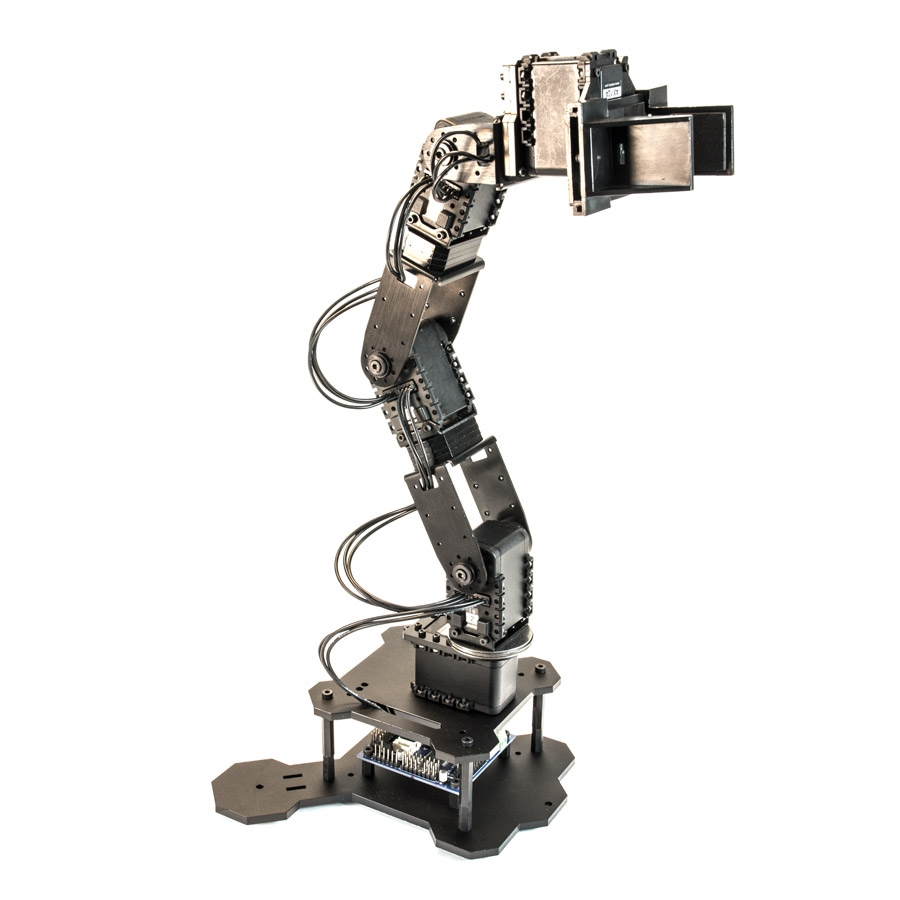
\includegraphics[width=10cm]{Robot.jpg}
	\caption{PhantomX Pincher Robot Arm}
	\label{fig:Robot_Trossen}    
\end{figure}
%% Origin: http://www.trossenrobotics.com/p/PhantomX-Pincher-Robot-Arm.aspx


\subsection{Specifications}
This robot has 5 degree of freedom. As it is a starter kit, the specification are designed for small applications only.

\begin{table}[h!]
\begin{tabular}[t]{|l |c|}\hline
Combination & Value \\
\hline 
\hline 
 Weight & 550G\\
 \hline 
 Vertical Reach & 35CM\\
 \hline 
 Horizontal Reach & 31CM\\
 \hline 
  & 25CM/40G\\
  Strength & 20CM/70G\\
  & 15CM/100G\\
  \hline 
 Gripper Strength & 500G/100G\\
 \hline 
 Wrist Lift Strength & 250G\\

\hline
\end{tabular}
\caption{Pincher Robotic Arm Specs} 
\label{tab:Arm_Specs}
\end{table}

As we can see in Table 1, this robot can not lift highly weighted objects, confirming the "starter kit" name. All the specifications needs to be taken in account for any application. If not, irreversible hardware damages can occur. 

\subsection{Aim}
The PhantomX Pincher Robot Arm can be used for many purposes. Its main advantage is being newbie-friendly, allowing non specialised users to have their own self-built robot. Using such a robot is also a great way to be introduced to the ROS (Robot Operating System) open source middle-ware. Skills in the ROS domain are more and more valuable from the companies point of view, as the 'language' is becoming very popular. Using ROS also brings the opportunity to improve Linux skills. In fact, ROS is considered stable on Linux (14.4) only. Linux may not appear as 'user friendly' as Windows on the first look, but once you get into it, you will see all the possibilities that are available to you. 
%%% check for US/EN

	
\subsection{Our opinion}
As we saw previously, this robot produced by Trossen Robotics is used to mimic a human arm. This robot is used mostly for learning purposes, therefore fitting our needs. But the limitations of such a robot are reached quite quickly. Indeed, this kit is designed for beginners, reducing a lot all the possibilities compared to other robots. For example, we would not recommend anyone to commercialize a project based on this robot, as it is imprecise and has a very limited strength. Overall, we think that learning everything, from building the robot to interfacing it with ROS.

	


\section{'Robot-Kit'}
\subsection{Arm design}

The arm can be simplified as 5 parts:

\begin{enumerate}
\item The base, composed of the deck, the arduino board and the shoulder pan motor
\item The shoulder lift motor
\item The elbow flex motor
\item The wrist flex motor
\item The gripper motor
\end{enumerate}


\begin{figure}[H]
	\centering
	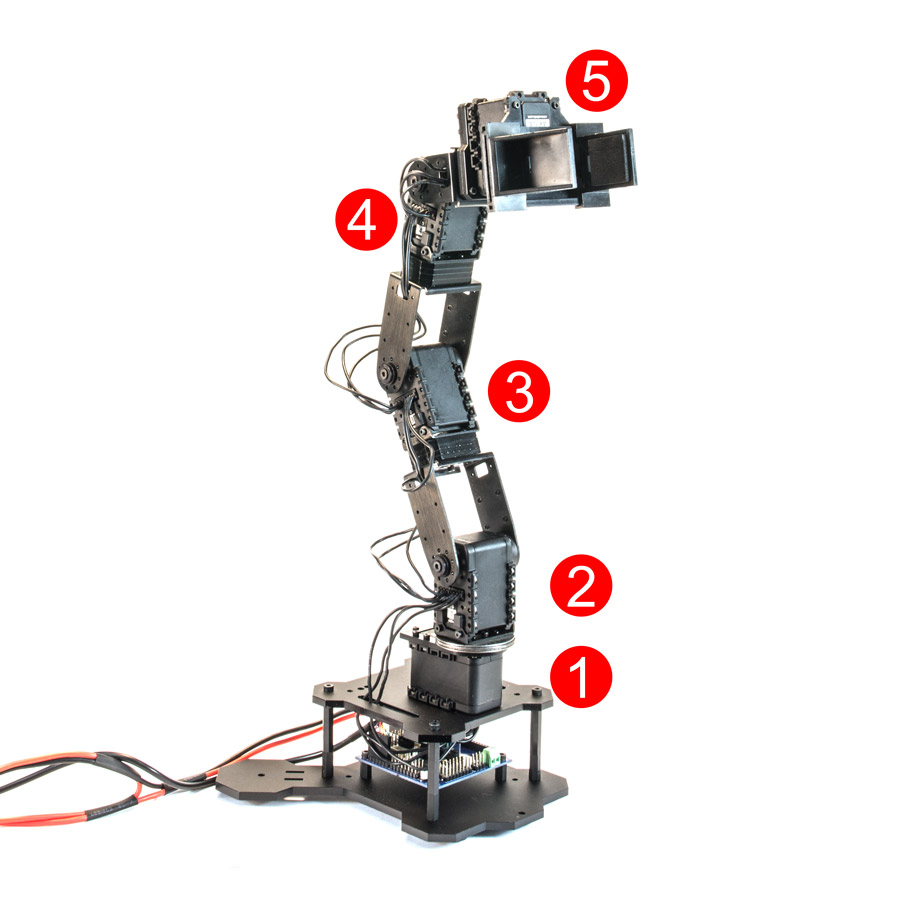
\includegraphics[width=10cm]{ArmNumbers.jpg}
	\caption{Parts of the arm}
	\label{fig:Armparts}    
\end{figure}
%%http://learn.trossenrobotics.com/images/assembly/phantomX-pincher/phantomxpinchernumbers.jpg



\subsection{Kit Overview}
In Figure 4 is presented the Kit on our workspace
\subsection{Kit Overview}

\begin{figure}[H]
	\centering
	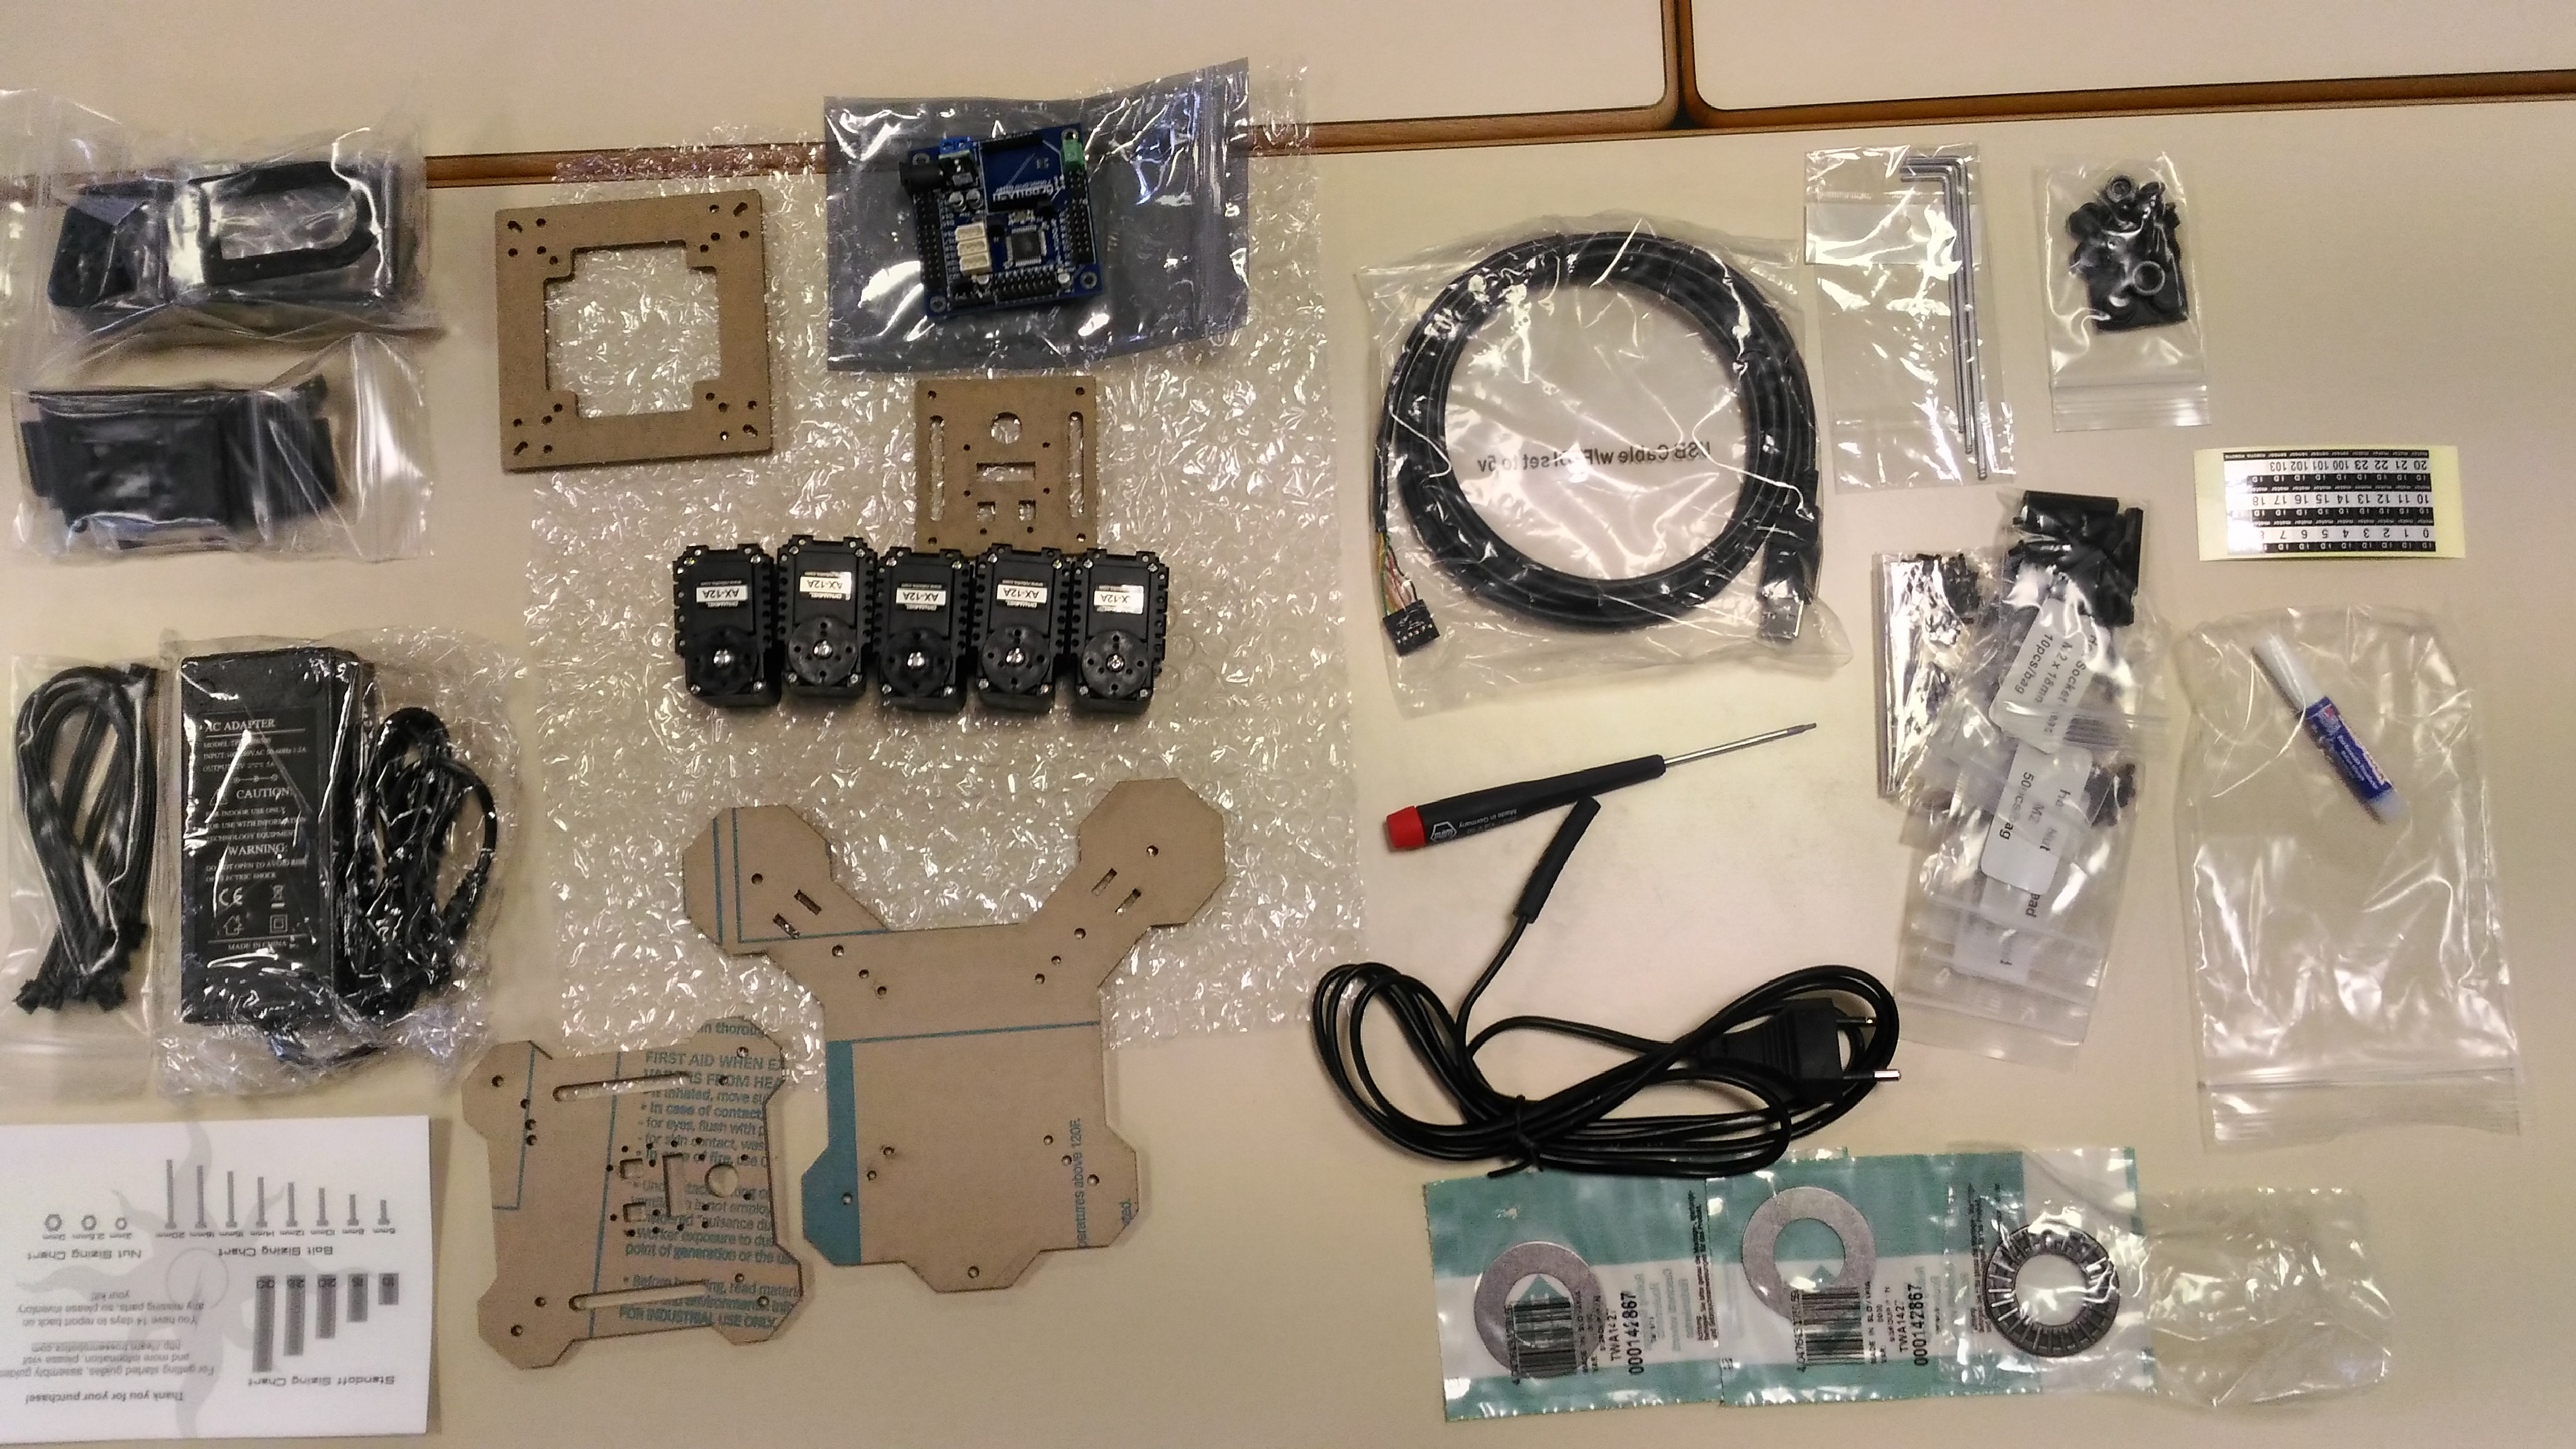
\includegraphics[width=10cm]{kit.jpg}
	\caption{Kit after opening}
	\label{fig:Kit}    
\end{figure}


\subsection{How to?}
\subsubsection{Defining the working environment}

In order to build the robotic arm, we had to organize our workplaces as well as possible.
To do this, we simply put together three tables in the center of the room, 
on which we gathered all the components to get an overview of the kit and start sorting the components.
Once done, we selected the different tools needed for the building process, such as glass to sort screws and nuts.
We chose to build the robot over two sessions, to not be in a rush but also to not take to much time for the building and forgot the current task.
We use a plastic glass to put little components inside during the building and we started this last one.
Finnally, we scheduled the work according moslty to the Trossen Rootics assembly guide [2]. The schedule is the following:
\begin{enumerate}
\item Perform the preliminary tasks
\item Install software and drivers, and set the servo IDs and centering
\item Build the three main parts of the robot (see Assembly)
\item Assemble those parts
\item Test and debug the robot
\end{enumerate}
So we started with the preliminary tasks

\subsubsection{Performing the preliminary tasks}

The main preliminary task concerned probably the nuts of this system. This product is quite a low cost one and we could see it when trying to place the nuts on the servos. According to the video included with the guide, placing them should have been a piece of cake. But the reality is that it took us two hours to figure out how to fix them properly and then place them.
In the kit was provided some glue, to better fix the components. We think it is wiser to note use it as the operations would therefore not be reversible. We are just begeinner in the field, and prefer to have to put some screw again rather than having a non fonctionnal piece. Therefore, we skipped this part.
In this part, we should also have sand the gripper rails. unfortunately, we did not saw it on the guide: we went to fast in the building process. So we did it after the assembly. But we would recommend anyone to perform this as a preliminary task as it is a waste of the to disassemble some part to assemble them again later.
Once these parts done, we could move to the sofware installations.

\subsubsection{Software installation}

All the software are installed on Ubuntu. This was a first challenge for use, as we are not familiar with this operating system. However, by being ressourceful, we managed to figure things out, such as the main console commands. The ones that we used the most are {chmod} for execution/read/write rights, {sudo} to perform tasks requireing admin rights, {apt-get} to directly instal some packages.
The first software we intalled is Arduino. We dowloaded mannualy a specific version as it is the only one a hundred percent compatible with our arduino board (Arduino 1.0.6). By placing it is our workspace folder, we could then start it just by using the {./Arduino} console command.
After that, we could skip the FTDI-2-USB drivers as the come directly with Ubuntu.Then, we included the Arbotix libraries in Arduino simply by placing them in the Arduino folder placed in {Documents}. Once done, we tried to make the Arduino board to blink and encoutered our first problem: we could not reach the board through USB. We found that the problem was access right. We fixed it by using {chmod} on the usb port. We were then able to run the Blink arduino sketch, meaning that we established communication with the board. Time to move to the servos IDs and centering.
For this part, a software called Dynamanager is required. This part took us some time due to our lack of knowledge on Ubuntu terminal commands and file management system. The main `trick' here is to not forget to make to Dynamixel file executable... We then used to software to set and the servos IDs and center them if the were not. We added some stickers on the servos to know which one is associated with which ID.
All the part being done, we could move to the assembly.

\subsubsection{Assembly}

As said previouly, we could split the building process (and therefore the robot) in three main parts:
\begin{enumerate}
\item The base, composed of the base servo and the shoulder lift servo;
\item The body of the arm, containing the elbow flex motorand the wrist flex motor;
\item The gripper
\end{enumerate}
\begin{figure}[h]
	\centering
	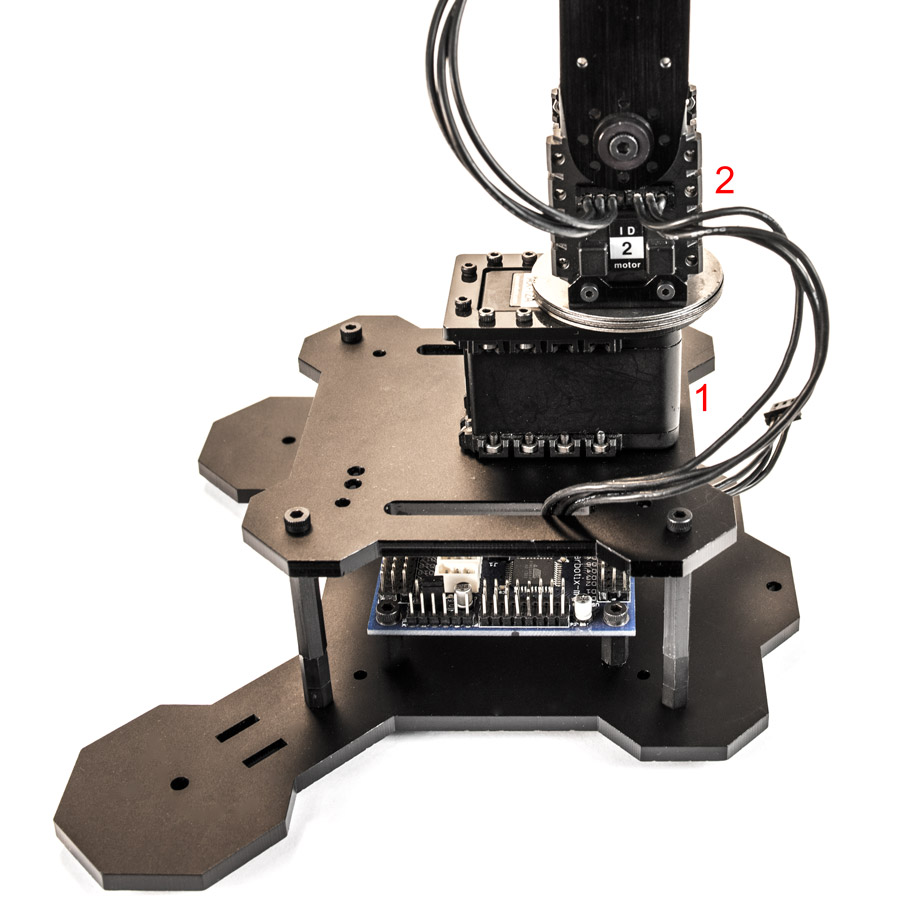
\includegraphics[height=8cm]{wire4.jpg}
	\caption{Base of the arm}
	\label{fig:Base}    
\end{figure}


For the first part, the base (Figure 5), we have built and unbuilt it four or five times later due to a bad sizing (hard to plug-in wires) and maybe an unprecision of the documentation. Building it once more again could now be done blindfolded.
For the body of the arm (Figure 6), we had to pay attention to the fixing of the robots. In fact, ti part will carry a lot of the mechanical weigth when usingthe robot, and we do not want it to overwhelm.
The last part is the gripper(Figure 7). For this one, we had to understand the moving system of two part with only one motor, as it was tricky to assemble it using the documentation only (as it is, once again, unprecise).
\begin{figure}[h]
	\centering
	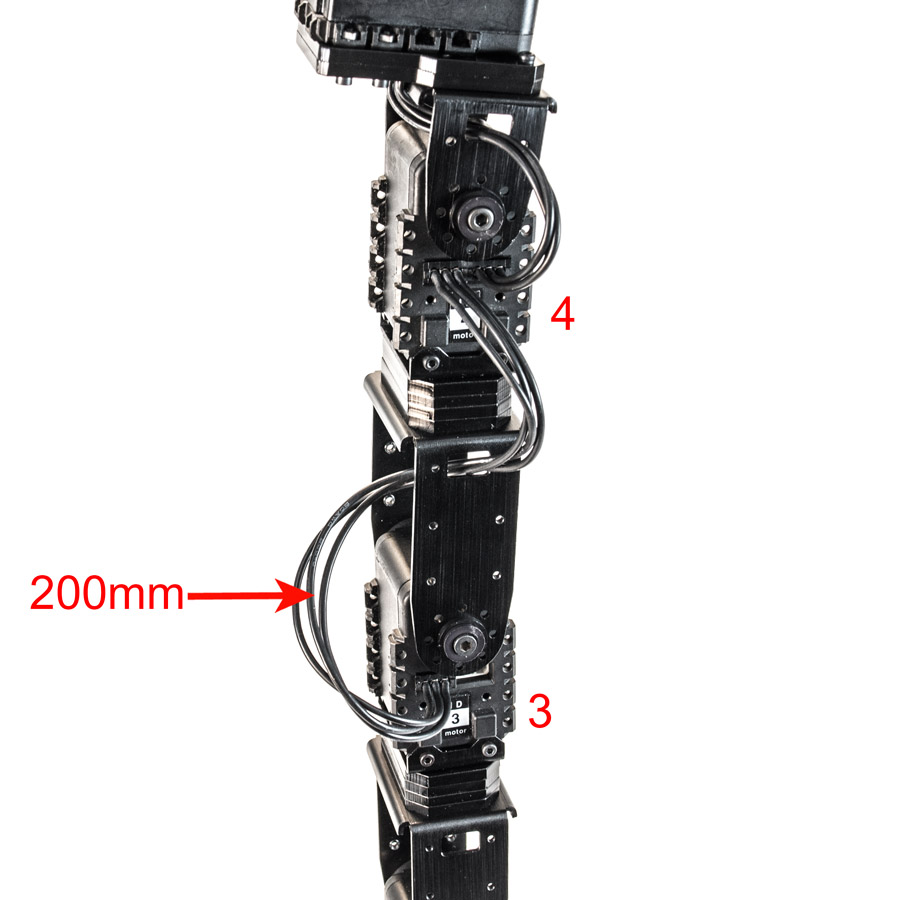
\includegraphics[height=8cm]{wire2.jpg}
	\caption{Body of the arm}
	\label{fig:Middle}    
\end{figure}

Finally, we could assemble those three parts and wire it together correctly, forming the final robot.

During the building process, we lost some time for two reasons. The first one is the lack of precision in the provided guide. In fact, some screw serial number were not matching between the guide and the kit. Therefore we had to replace that with other, checking that we would not need them for a later use. The second time consuming issue was our lack of experience in building robots. Even tho we tried to follow the guide as much as possible, we did mix a bit the ordering, and had to dismout and mount again some pieces of the robot. We consider it a part of the learning process, and hope we will be able to avoid such mistakes in the future.
\begin{figure}[H]
	\centering
	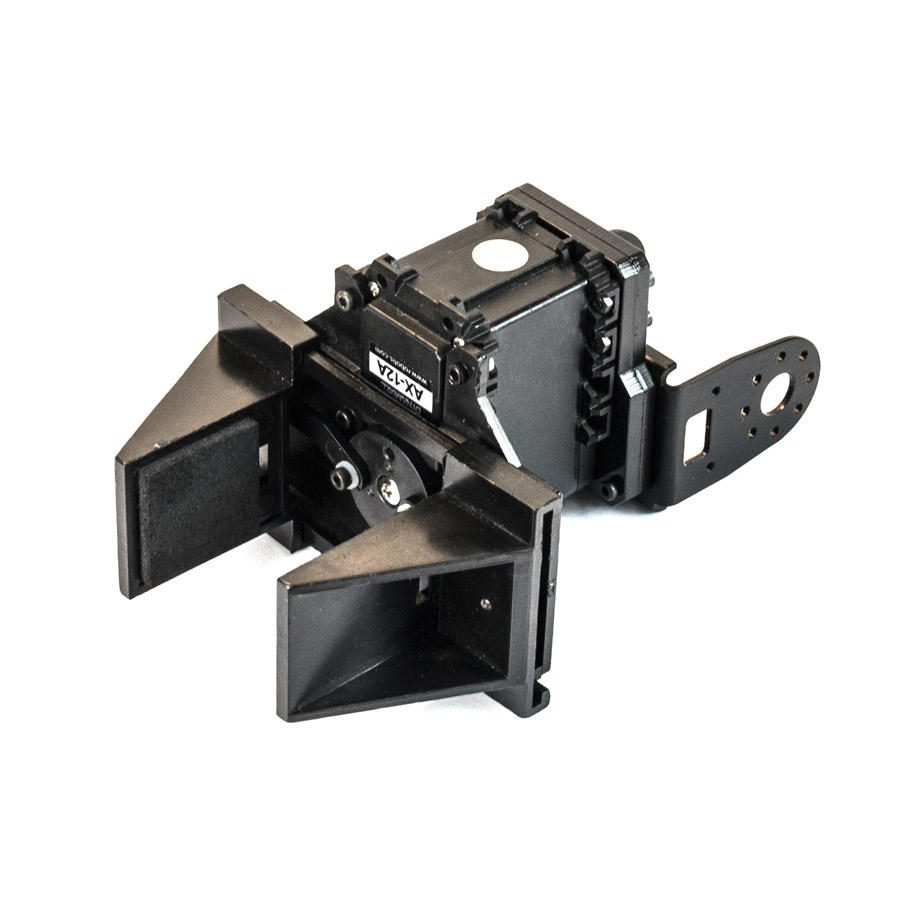
\includegraphics[height=8cm]{grip4.jpg}
	\caption{Gripper}
	\label{fig:Gripper}    
\end{figure}

The assembly was a very interesting (and somehow quite fun) part of this project. Time to try the robot !

\subsubsection{Debugging using Arduino}
Well... not really. We tend to forget this last part, but this is mandatory. The ArbotiX sketchbook come with code to debug and try the robot motors using Adurino serial terminal. Here we encoutered one more problem : the "Voltage levels below 10v, please charge battery". The guide states that it could occur if the power supply is no sufficient or if the servo IDs were not set properly. As we used the power supply provided with the kit, and as the board jumpers were set properly, it had to come from the servo IDs. It was a surprise to us as we took quite some time to double check taht the IDs were properly set and the wires connected as stated on the guide. But as mistakes can happends, we performed to ID stting part agin (meaning debuilding the robot). Even after that, we still had the same error message. By trying several things, we figured out something that was not said in the guide: the wire might be a bit loose. so you have to `play' with it until it works. Once the error remove, some of our servos were not moving. Once again, the provided documentation led to some errors: the wires connection on the servos (left or right) was not the good one. After fixing it by trying, we finally managed to have a fully working robot.

\subsection{Challenges encountered}
During this project, we face several challenges:
\begin{itemize}
  \item Our lack of knowledge on Ubuntu. This project helped us a lot to understand Unbuntu and its features.
  \item Ourselves. Indeed, we were really hyped by the project and sometimes, we were going to fast, skipping important parts of the building process.
 \item The documentation. We do not understand how can a documentation of a commercial product contain so much imprecision (software versions for example). We had to be ressourceful to figure out by ourselves how to perform some tasks.
\end{itemize}

Overall, we think that this project was a great idea to introduce us to the robotics field, as we learnt a lot of different skills.

\section{ROSification}
During the semester, we will use ROS to control robots. However, at this stage we do not know much about ROS. The comming lessons will allow us to understand it better, and maybe interface the robot with it. This is why we chose to not try to interface it by ourselves. It would have taken too much time for a poor result. But as kids with there new toys, we wanted to `play' with the arm, and control it with ROS. By some researches, we found a simple but great tutorial [3] with provided packages [4] to perform it. This packages contains a GUI to control separatly each servo. At this stage, we tweaked the package on simple things such as maximum rotation of each servo and changing the GUI. With not that much success. ROS is still to foggy for us.

\section{Future plan}
As the arm is now functionnal and as we know that it could be interfaced with ROS, one could use it as a plugin for the Kuboky TurtleBot ( some components from the arm kit remain unused). For the next year, a good project could be to do this building in view of control the Turtle bot and the arm at the same time. Using this improvement, one could control the turtle bot, pickup up an object which take place anywhere in the room and bring up in an another place. By keyboard, joystick or programing, every means could be use to do this combo. One could even use the Kinect to detect object matching specific feature and place it in the room according the the objects' shape. With a TurtleBot and sucha  plugin, the possibilites are endless!


\section{Conclusion}
There is no doubt: we enjoy the project. We would like to thank the Professors for coming up with such an idea and finding the way to make it possible (found, time, ...). We think that being introduce to the field in such a way is far better than endless theoretical lessons. We do not deny importance of the theoretical part, but learning while having fun is great. 
This project allowed us to understand the very basics of ROS (works with packages), improve our knowledge of the Ubuntu operating system and also rething our working methods with the kit building. 

\section{Bibliography}
\begin{enumerate}
\item \href{http://www.trossenrobotics.com/p/PhantomX-Pincher-Robot-Arm.aspx}{Arm page}

\item \href{http://learn.trossenrobotics.com/16-interbotix/robot-arms/pincher-robot-arm/163-phantomx-pincher-robot-arm-assembly-guide.html}{Assembly guide}

\item \href{http://www.iroboapp.org/index.php?title=Getting_Started_with_Turtlebot_Arm_PhantomX_Pincher_with_ROS}{ROSification guide}

\item \href{https://github.com/turtlebot/turtlebot_arm}{Ros interface source code}
\end{enumerate}

\end{document} % DONE WITH DOCUMENT!